\section{แนวคิดและวิธีการดำเนินงาน}

งานวิจัยนี้นำเสนอวิธีการสร้างกรณีทดสอบและข้อมูลทดสอบสำหรับ{\TestPath}ระหว่าง{\CUT}อย่างน้อย 1 เส้นทาง 
บน{\StaticInformation}จาก{\sourcecode}ภาษาจาวาตามที่ผู้ทดสอบสนใจ โดยมีภาพรวมการดำเนินงานวิจัย 
ดัง\figref{fig:methodologyoverview} ซึ่งมีแนวทางการดำเนินงานดังนี้

\begin{sidewaysfigure}
    \centering
    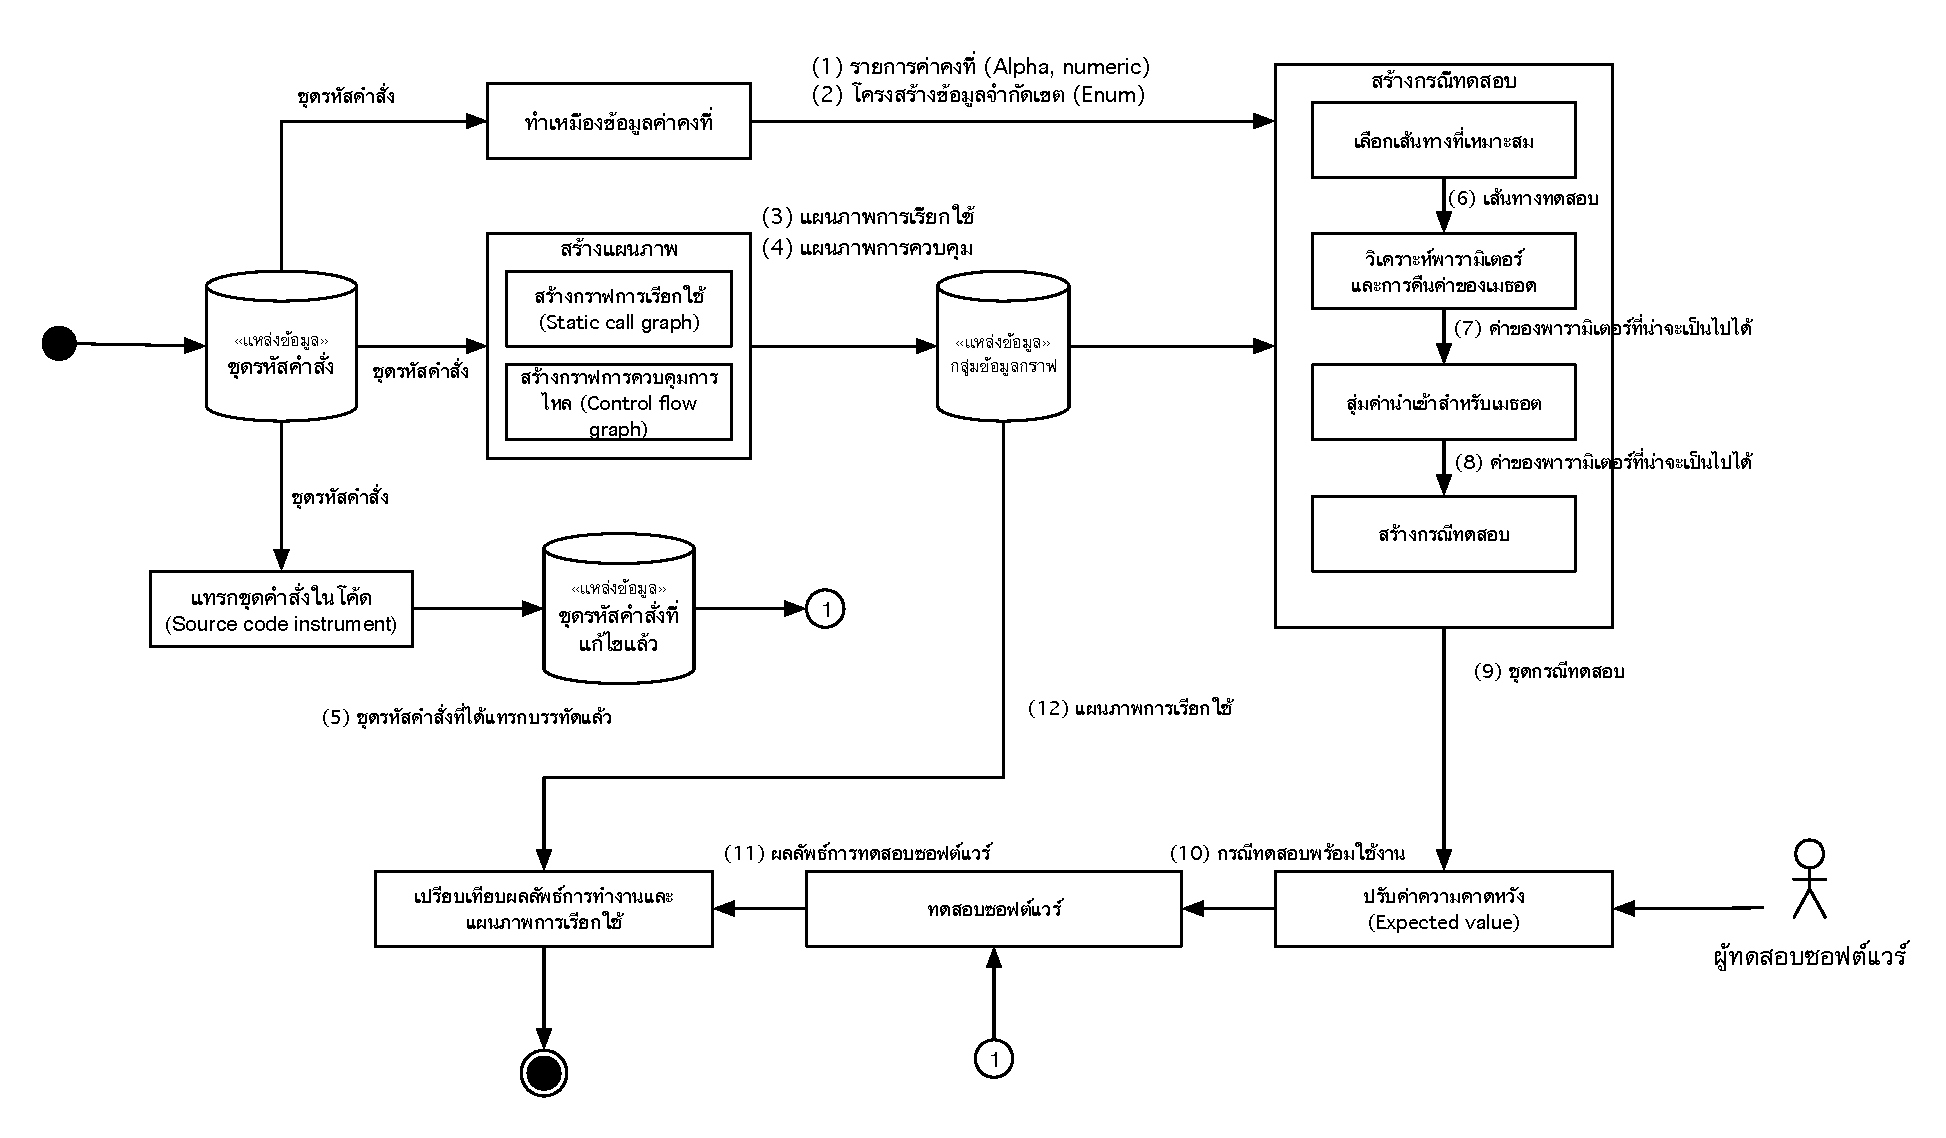
\includegraphics[width=0.9\textwidth]{methodology-overview}
    \caption{ภาพรวมการดำเนินงานวิจัย}
    \label{fig:methodologyoverview}
\end{sidewaysfigure}

\subsection{การวิเคราะห์ข้อมูลเบื้องต้น}

ในขั้นตอนนี้เริ่มต้นด้วยการนำเข้าข้อมูล{\sourcecode}จาก{\Repository} เพื่อนำมารวบรวม{\StaticInformation} 
โดยสนใจเพียงเฉพาะ{\class}ซึ่งบรรจุอยู่ภายในกลุ่มข้อมูล (Package) ตามที่ผู้ใช้งานระบุ กำหนดให้เป็น "\FirstTimeDefine{\CUT}{\CUTEN}" 
ทั้งนี้กระบวนการจะประกอบไปด้วย 3 ขั้นตอนด้วยกัน นั่นคือ
{\bf การทำเหมืองข้อมูลค่าคงที่ (2)}, {\bf การสร้างกราฟ (3)} และ{\bf การแทรกชุดคำสั่งใน{\sourcecode} (4)} โดยมีแนวทางการดำเนินงานของแต่ละขั้นตอน 
ดังนี้

\subsubsection{การทำเหมืองข้อมูลค่าคงที่ (2)}

การทำเหมืองข้อมูลค่าคงที่นั้นเป็นกระบวนการเพื่อกำหนดแนวทางการในการสร้างข้อมูลทดสอบสำหรับ{\TestPath}ที่เลือก โดยมีแนวทางการจัดเก็บค่าคงที่ที่ประกาศไว้
ภายใน{\sourcecode} โดยสนใจกลุ่มข้อมูล 2 กลุ่ม ได้แก่

\begin{enumerate}
    \item ข้อมูลพื้นฐาน (Primitive data) {\it (ก)} ซึ่งเป็นข้อมูลพื้นฐานที่ใช้งานภายใน{\class} ซึ่งในที่นี้จะสนใจข้อมูลพื้นฐาน 2 ประเภทได้แก่
        \begin{enumerate}
            \item {\bf ตัวอักษร} ซึ่งมีประเภทข้อมูลเป็น {\it String} ในภาษาจาวา
            \item {\bf ตัวเลข} ซึ่งมีประเภทข้อมูล ได้แก่ {\it byte}, {\it short}, {\it int}, {\it long}, {\it float} 
               และ {\it double} ในภาษาจาวา
        \end{enumerate}
    \item โครงสร้างข้อมูลจำกัดเขต (Enumeration) {\it (ข)} ซึ่งมีประเภทข้อมูลเป็น {\it enum} ในภาษาจาวา
\end{enumerate}
% (String) ตัวเลข (Number) ซึ่งมีประกอบไปด้วยข้อมูลประเภท byte, short, int, long, float และ double และชุดข้อมูล (Enumeration) 

ทั้งนี้จะไม่สนใจข้อมูลเชิงตรรกะ (มีชนิดข้อมูลเป็น {\it bool} ในภาษาจาวา) เนื่องมาจากว่าตัวเลือกที่เป็นไปได้จำกัดอยู่แล้ว 
นอกจากนั้นจะยังไม่สนใจข้อมูลจำเพาะ ที่กำหนดขึ้นมาใช้งานเอง 

หลังจากรวบรวมค่าคงที่จาก{\sourcecode}ได้เรียบร้อยแล้ว จะนำ{\bf ข้อมูลพื้นฐาน (ก)} และ{\bf โครงสร้างข้อมูลจำกัดเขต (ข)} ที่รวบรวมได้
จัดหมวดหมู่และบันทึกไว้ภายใน{\it ฐานข้อมูล (A)}

\subsubsection{การสร้างกราฟ (3)}

กระบวนการสร้างกราฟนั้นจะรับข้อมูล{\sourcecode}จาก{\Repository}เพื่อนำข้อมูลมาใช้สร้างกราฟ โดยแบ่งออกเป็น 2 กระบวนการย่อยด้วยกัน 
นั้นคือ การสร้าง{\scg} และการสร้าง{\cfg} ดังนี้

\begin{enumerate}
    \item {\bf สร้าง{\scg}} อ่านข้อมูล{\CUT}ตามที่ผู้ใช้งานสนใจ แล้วนำมาสร้าง{\scg} โดยผลลัพธ์ที่ได้นั้นจะแบ่งเป็น 3 กลุ่ม ได้แก่
        \begin{enumerate}
            \item การเรียกใช้งานระหว่าง{\CUT}ด้วยกัน \label{ord:scgcut}
            \item การเรียกใช้งานระหว่าง{\CUT}และ{\class}ภายในชุดพัฒนาของจาวา (Java SDK) \label{ord:scgjdk}
            \item การเรียกใช้งานระหว่าง{\CUT}และชุดคำสั่งภายนอก (3$^{rd}$ party library) \label{ord:scg3rd}
        \end{enumerate}
        ซึ่งในแนวทางการดำเนินงานนี้จะสนใจเฉพาะ{\scg}ของ{\CUT}เท่านั้น ดังนั้นในขั้นตอนนี้ไม่สนใจกราฟที่เกิดจากการเรียกใช้ในข้อ \ref{ord:scgjdk} 
        และ \ref{ord:scg3rd} ตลอดจนกราฟที่เกิดจากการสร้างวัตถุใหม่ เพื่อให้ได้{\scg}เฉพาะ{\CUT} ดังเช่น \figref{fig:scggrading}

    \item {\bf สร้าง{\cfg}} โดยจะอ่านข้อมูลของ{\CUT}นำมาสร้าง{\cfg}และจัดเก็บข้อมูลไว้ภายในฐานข้อมูล
\end{enumerate}

เมื่อสิ้นสุดกระบวนการจะนำข้อมูล{\bf {\scg} (ค)} และ{\bf {\cfg} (ง)} ที่ได้จัดเก็บลง {\it ฐานข้อมูล (A)} เพื่อจัดเตรียมไว้สำหรับ 
{\bf ขั้นตอนการสร้างกรณีทดสอบ (5)} และ{\bf เปรียบเทียบผลลัพธ์การดำเนินการ (8)} ต่อไป

\subsubsection{การแทรกชุดคำสั่ง (4)}

เนื่องจากว่าการทดสอบนี้จำเป็นต้องครอบคลุม{\Path}ระหว่าง{\CUT} ดังนั้นจำเป็นจะต้องแทรกชุดคำสั่งใน{\sourcecode}ในแต่ละขั้นตอนการทำงาน 
(Code instrument) จากนั้นจึงนำ{\sourcecode}ที่ผ่านการแทรกชุดคำสั่งเรียบร้อยแล้วไปใช้ในกระบวนการทดสอบ 
แล้วจึงจัดเก็บผลลัพธ์ที่ได้ระหว่างขั้นตอนการทดสอบ เพื่อนำมาเปรียบเทียบกับ{\TestPath}ที่เลือก

\begin{figure}[hbt!]
    \lstset{style=thesiscodestyle}
    \lstinputlisting[language=java]{methodology/SimpleBonusScoreInstrumented.java}
    \caption{{\class} \code{SimpleBonusScoreInstrumented}}
    \label{fig:javaBonusScoreInstrumented}
\end{figure}

จากตัวอย่าง\figref{fig:javaBonusScoreInstrumented} เป็น{\sourcecode}ที่สืบเนื่องมาจาก\figref{fig:javaBonusScore}
แต่ต่างกันโดยแทรกชุดคำสั่งเข้าไปภายใน{\sourcecode} ณ บรรทัดที่ 5, 10, 13 และบรรทัดที่ 18 ซึ่งการแทรกชุดคำสั่งในกระบวนการนี้จะสนใจเพียงแค่{\CUT} เท่านั้น

เมื่อเสร็จสิ้นกระบวนการแทรกชุดคำสั่ง จะนำ{\sourcecode}ที่ได้จัดเก็บไว้ใน {\it ฐานข้อมูล (A)} เพื่อจัดเตรียมไว้สำหรับนำไปทดสอบอีกครั้ง

\clearpage
\subsection{การสร้างกรณีทดสอบ (5)}

การดำเนินงานวิจัยในครั้งนี้จะนำข้อมูลกราฟ (3) ซึ่งประกอบไปด้วยข้อมูล {\it {\scg} (ค)} ร่วมกับ{\it {\cfg} (ง)} ใช้เป็นข้อมูลเริ่มต้นสำหรับการหา{\TestPath}
ระหว่าง{\CUT} อย่างน้อย 1 เส้นทางระหว่าง{\class} แล้วจึงสร้างข้อมูลนำเข้าโดยพิจารณาจาก{\PredicateNode}ที่ปรากฎบน{\TestPath}ที่เลือก 
สุดท้ายจึงนำข้อมูลทั้งหมดที่ได้สร้างเป็นชุดกรณีทดสอบ โดยมีภาพรวมการดำเนินงานดัง {\figref{fig:testcaseGenerationActivity}}

\begin{figure}[ht!]
    \centering
    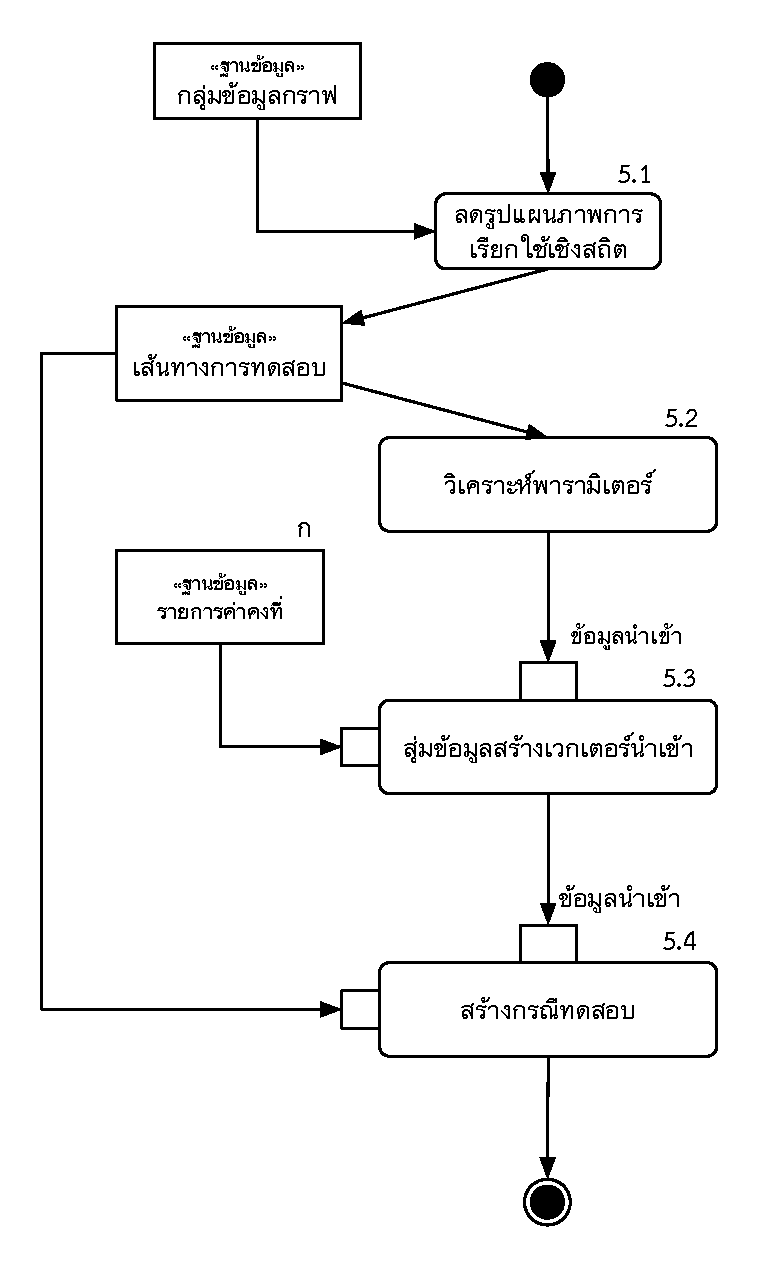
\includegraphics[width=0.5\textwidth]{methodology-activities-test-case-gen}
    % 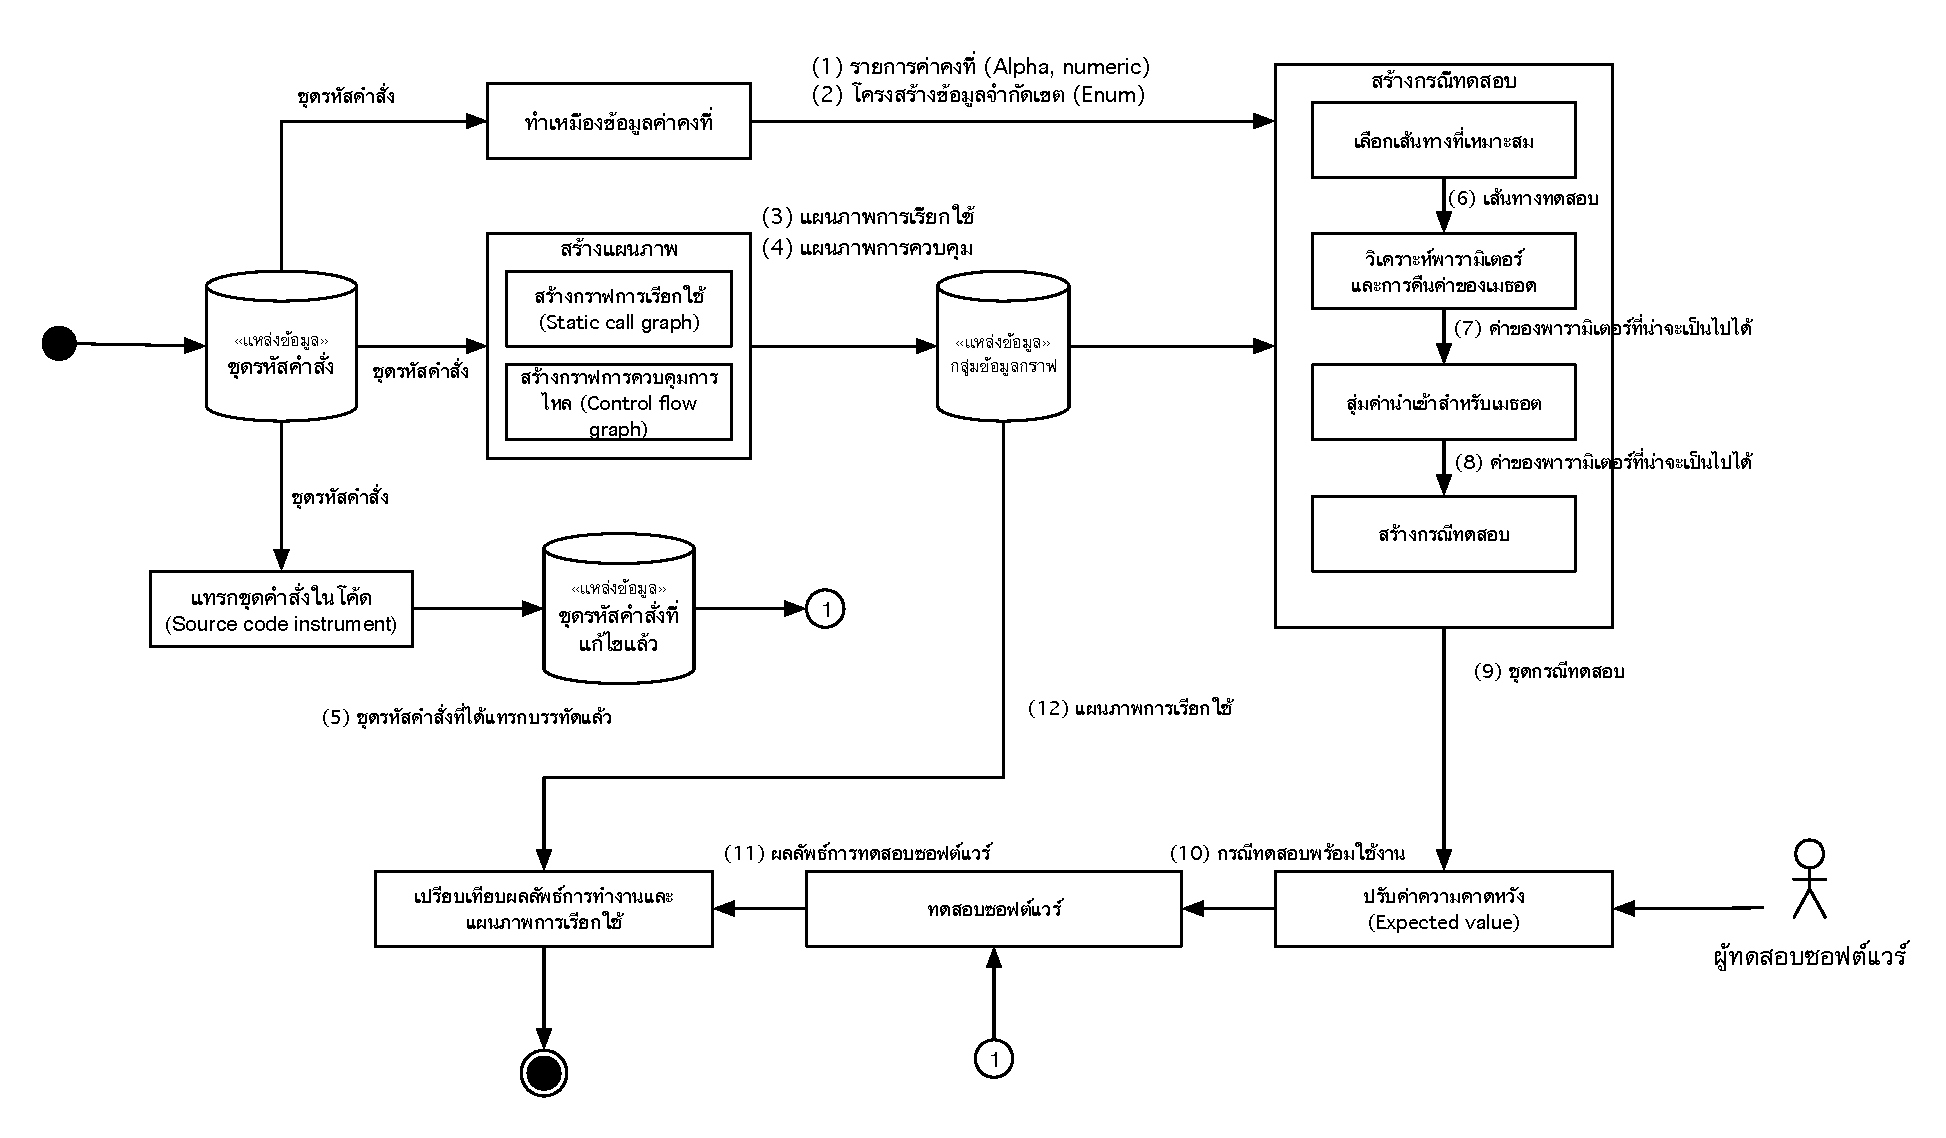
\includegraphics[width=0.9\textwidth]{methodology-overview}
    \caption{ขั้นตอนการสร้างกรณีทดสอบ}
    \label{fig:testcaseGenerationActivity}
\end{figure}

\subsubsection{เลือก{\TestPath} (5.1)}

ในขั้นตอนนี้จะพิจารณาจากข้อมูล{\it \scg (ก)} ร่วมกับ {\it \cfg (ข)} เพื่อเลือก{\TestPath}ที่ยาวที่สุดที่จะเป็นไปได้ใน{\scg} 
ในกรณีที่ระหว่าง{\CUT}นั้นมี{\Path}เชื่อมต่อกันมากกว่า 1 {\Path} จะกำหนดน้ำหนักให้กับ{\Edge}ของ{\scg} โดยพิจารณาจากจำนวนการเรียกใช้งานที่พบภายใน{\cfg} 
ตัวอย่างเช่น ระหว่าง\class\ \figref{fig:javaQuiz} และ\figref{fig:javaBonusScore} นั้นพบการเชื่อมต่อระหว่างกัน 2 {\method} นั่นคือ
\code{getQuizScore} และ\ \code{getQuizSum} แต่จากการพิจารณาใน{\sourcecode}พบว่า{\class}\ \code{SimpleBonusScore} นั้นเรียกใช้งาน\method
\code{getQuizScore} รวมทั้งสิ้น 2 ครั้ง ในขณะที่มีการเรียกใช้งาน \code{getQuizSum} เพียง 1 ครั้ง ดังนั้นจะได้{\scg}ที่ถ่วงน้ำหนักบน{\Edge}เรียบร้อยแล้วดัง 
\figref{fig:scgWeightedEdge}

ซึ่งจะได้{\scg}ของทั้ง 3 {\class}นี้เป็น

\begin{figure}[ht!]
    \centering
    \begin{minipage}{.8\textwidth}
        \centering
        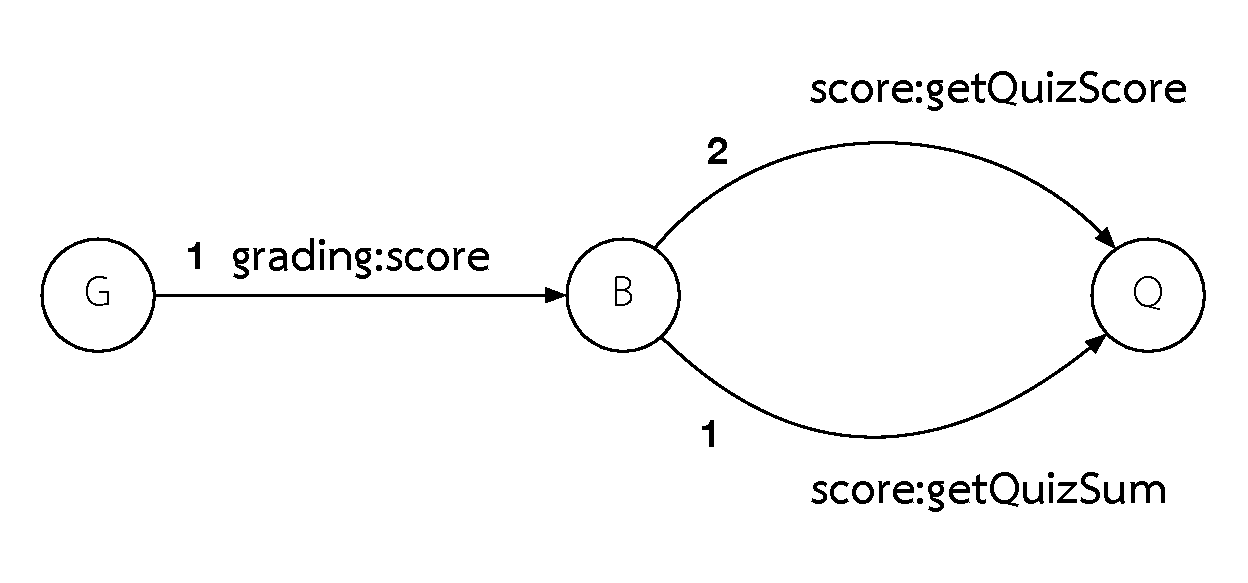
\includegraphics[width=0.8\textwidth]{scg-weighted-edges}
        \subcaption{{\scg}ถ่วงน้ำหนัก}
        \label{fig:scgWeightedEdge}
    \end{minipage}
    \begin{minipage}{.8\textwidth}
        \centering
        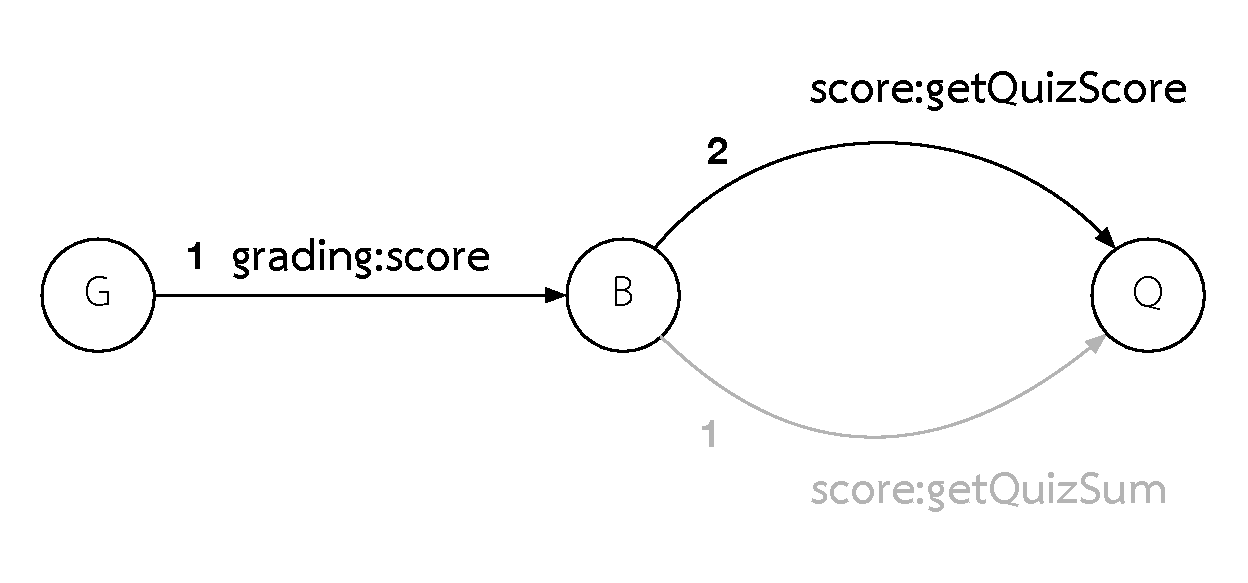
\includegraphics[width=0.8\textwidth]{scg-weighted-edges-testpath}
        \subcaption{\TestPath\ ที่เลือก}
        \label{fig:scgWeightedEdgeTestPathSelected}
    \end{minipage}
    \caption{{\scg}สำหรับโปรแกรมคำนวณเกรดนิสิต}
    \label{fig:scgCallGraph}
\end{figure}

ดังนั้น {\TestPath}ที่เลือกระหว่าง \code{SimpleBonusScore} และ \code{SimpleQuiz} คือ{\Path}ที่\class\ \code{SimpleBonusScore} 
เรียกใช้งาน{\method}\ \code{getQuizeScore} ดัง\figref{fig:scgWeightedEdgeTestPathSelected} ซึ่งมีแนวทางการเลือก{\TestPath} ดังนี้

\begin{enumerate}
    \item ให้น้ำหนักในทิศทางที่มุ่งไปยัง{\Node} ซึ่งพบการเรียกใช้งานระหว่าง{\class}ตามที่กำหนดไว้จาก{\scg}มากที่สุดเสมอ
    \item เลือก{\TestPath}ที่สั้นที่สุดก่อนเสมอ
    \item เลือก{\TestPath}ที่พบ{\PredicateNode}น้อยที่สุดก่อนเสมอ
    \item เลือก{\TestPath}ไปยังทิศที่ทำให้{\PredicateNode}มีค่าความจริงเป็นจริงก่อนเสมอ
\end{enumerate}

เมื่อพิจารณา{\cfg}ของ{\class}\ \code{SimpleGrading} และ \code{SimpleBonusScore} ดัง{\figref{fig:cfgSimpleGrade} 
และ\figref{fig:cfgSimpleBonusScore} ตามลำดับ พบว่า\code{SimpleGrading} ได้เรียกใช้งาน{\method} \code{score} ของ\class\ 
\code{SimpleBonusScore}\ ที่{\Node} 18 เรียบร้อยแล้ว จึงเลือก{\TestPath}ที่สั้นที่สุดภายใน {\code{SimpleGrade}} นั่นคือ 
17\ \textendash\ 18\ \textendash\ 19\ \textendash\ 20 \textendash\ 25\ \textendash\ 26 

ถัดมาจึงพิจารณา{\TestPath}ระหว่าง \code{SimpleBonusScore} และ \code{SimpleQuiz} ณ ตำแหน่งที่พบการเรียกใช้งาน \code{getQuizScore}
ซึ่งพบที่{\Node} 11 และ 16 หากเลือกเส้นทางทดสอบ เมื่อพิจารณาจากแนวทางด้านบนแล้ว จะได้{\TestPath} คือ 6\ \textendash\ 7\ \textendash\ 8\ 
\textendash\ 9\ \textendash\ 10\ \textendash\ 11\ \textendash\ 12\ \textendash\ 13\ \textendash\ 14\ \textendash\ 21\ 
\textendash\ 22\ \textendash\ 24 

โดยมี{\it {\TestPath} (ฉ)} ที่เลือก ดัง\tabpageref{tab:testPath}

\begin{table}[ht!]
    \centering
    \caption{{\TestPath}ที่เลือกโดยพิจารณาจาก{\scg}ร่วมกับ{\cfg}}
    \label{tab:testPath}
    \begin{tabular}{|l|l|}
        \hline
        \code{SimpleGrading}    & 17\ \textendash\ 18\ \textendash\ 19\ \textendash\ 20 \textendash\ 25\ \textendash\ 26 \\ \hline
        \code{SimpleBonusScore} & {\small 6\ \textendash\ 7\ \textendash\ 8\ \textendash\ 9\ \textendash\ 10\ \textendash\ 
                                    11\ \textendash\ 12\ \textendash\ 13\ \textendash\ 14\ \textendash\ 21\ \textendash\ 
                                    22\ \textendash\ 23\ \textendash\ 24}  \\ \hline
    \end{tabular}
\end{table}

\begin{figure}[ht!]
    \centering
    \centering
    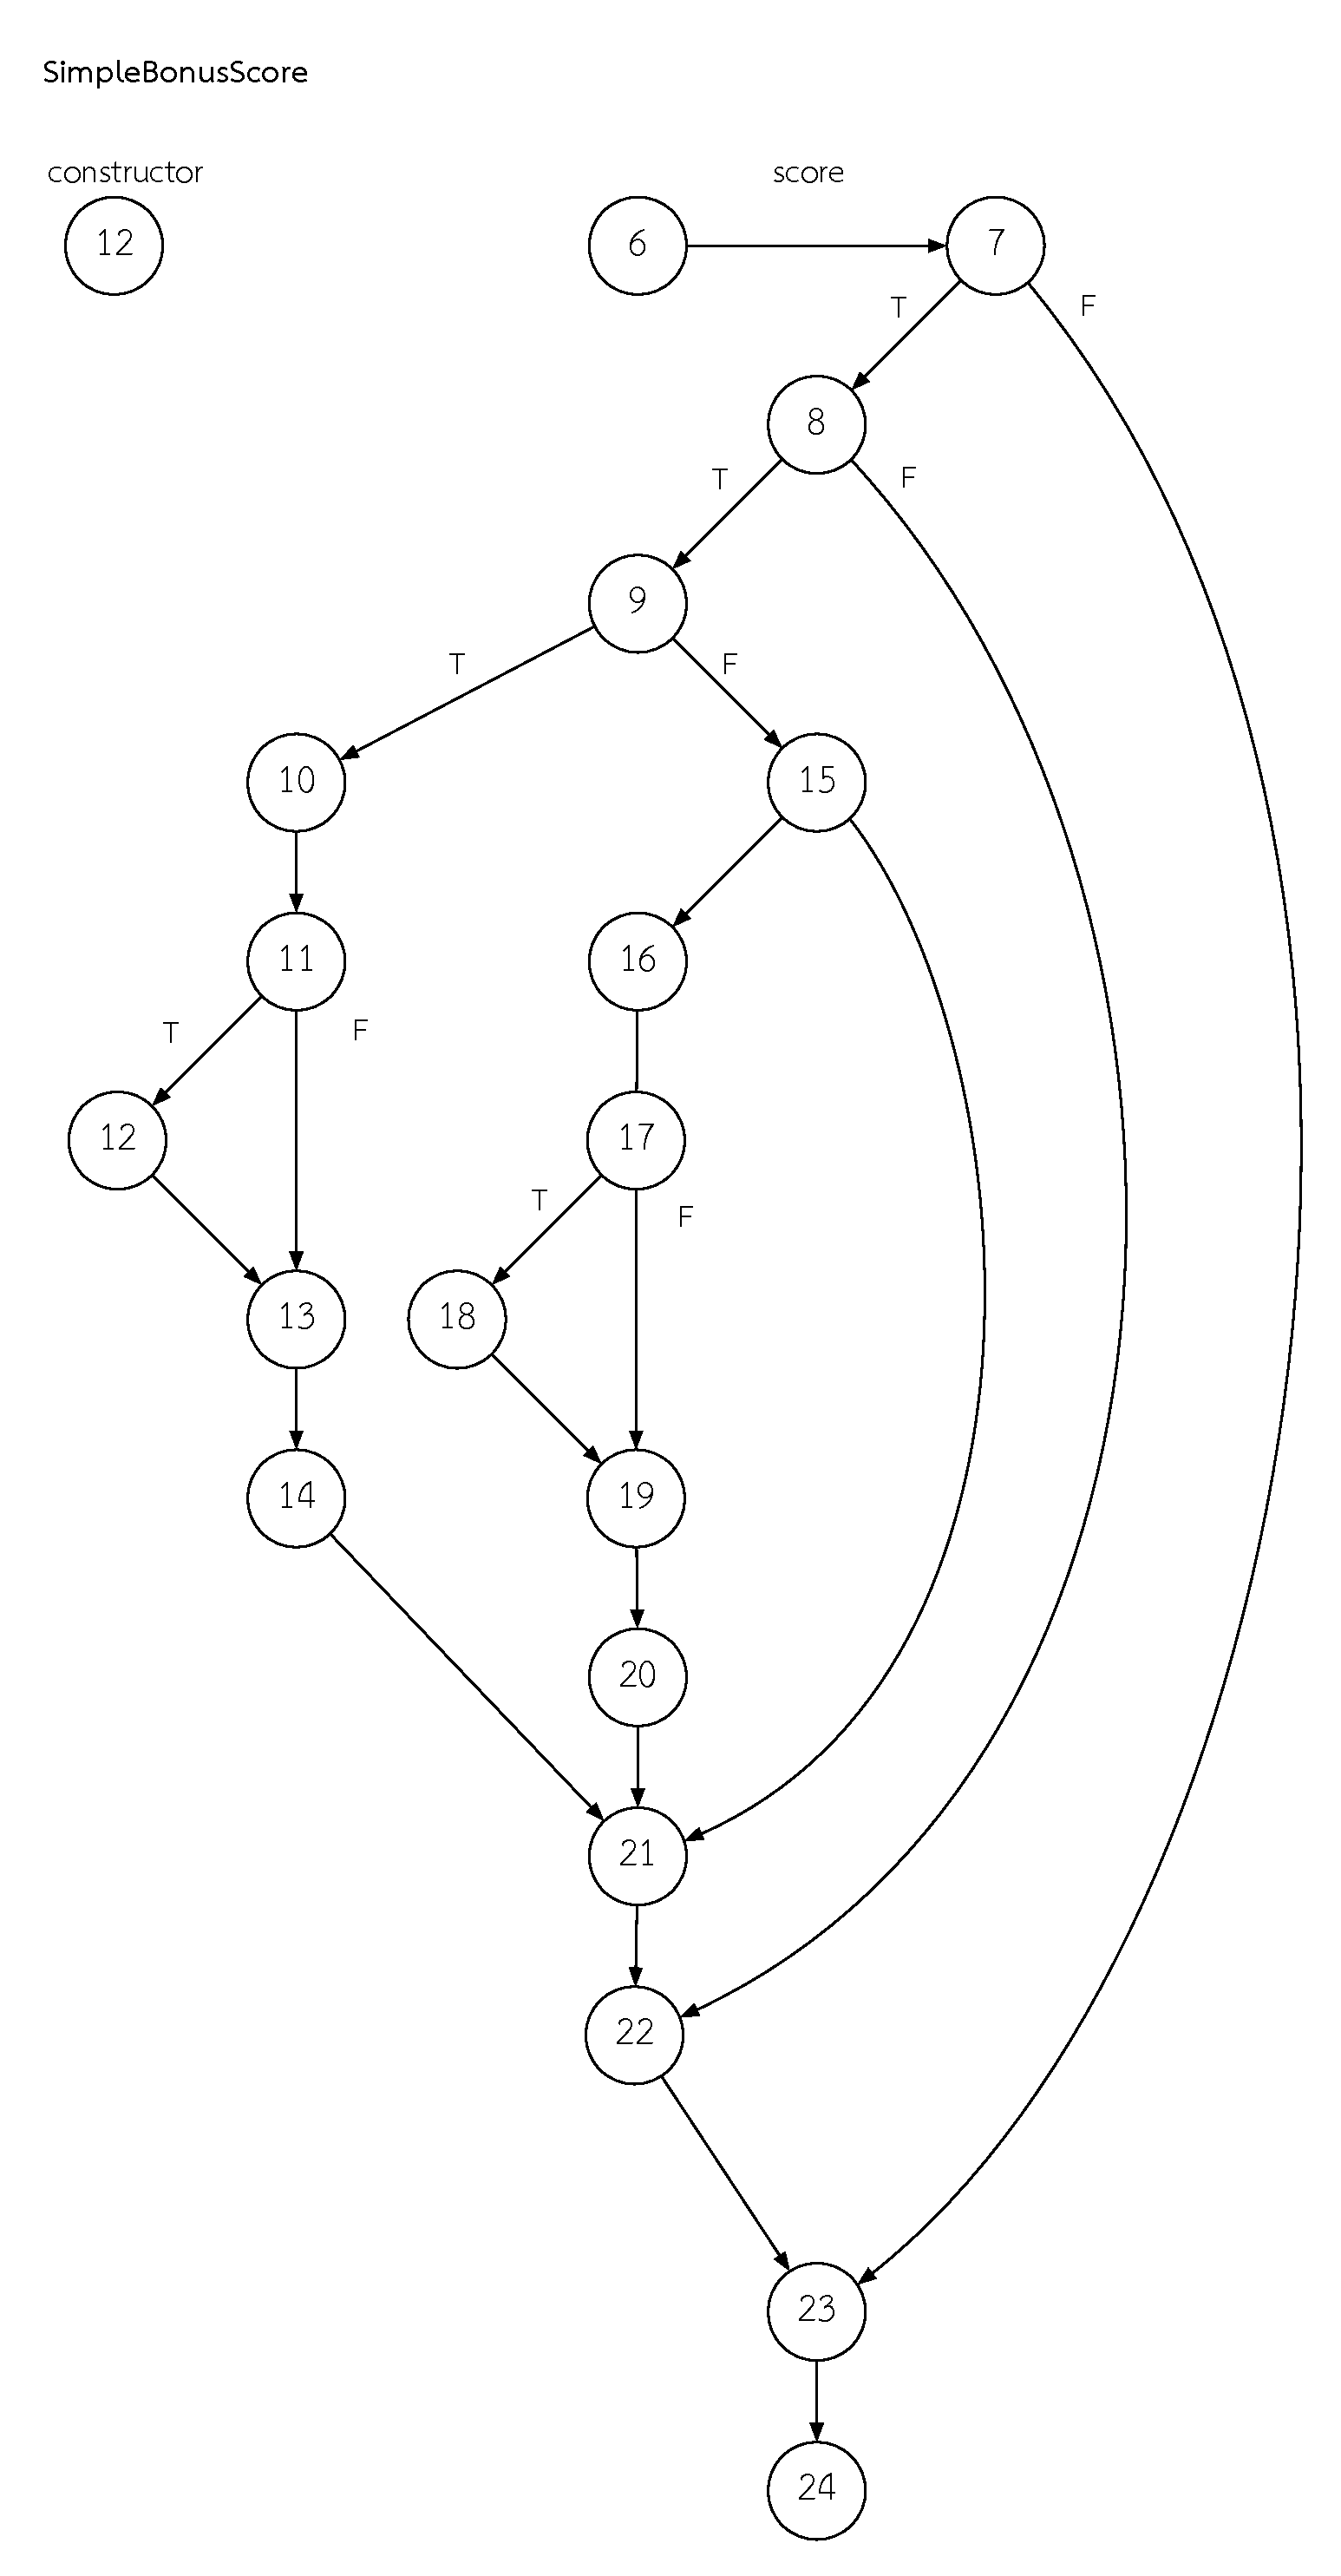
\includegraphics[width=0.7\textwidth]{cfg-SimpleBonusScore}
    \caption{{\cfg}สำหรับ{\class}คำนวณคะแนนพิเศษ}
    \label{fig:cfgSimpleBonusScore}
\end{figure}

\begin{figure}[ht!]
    \centering
    \centering
    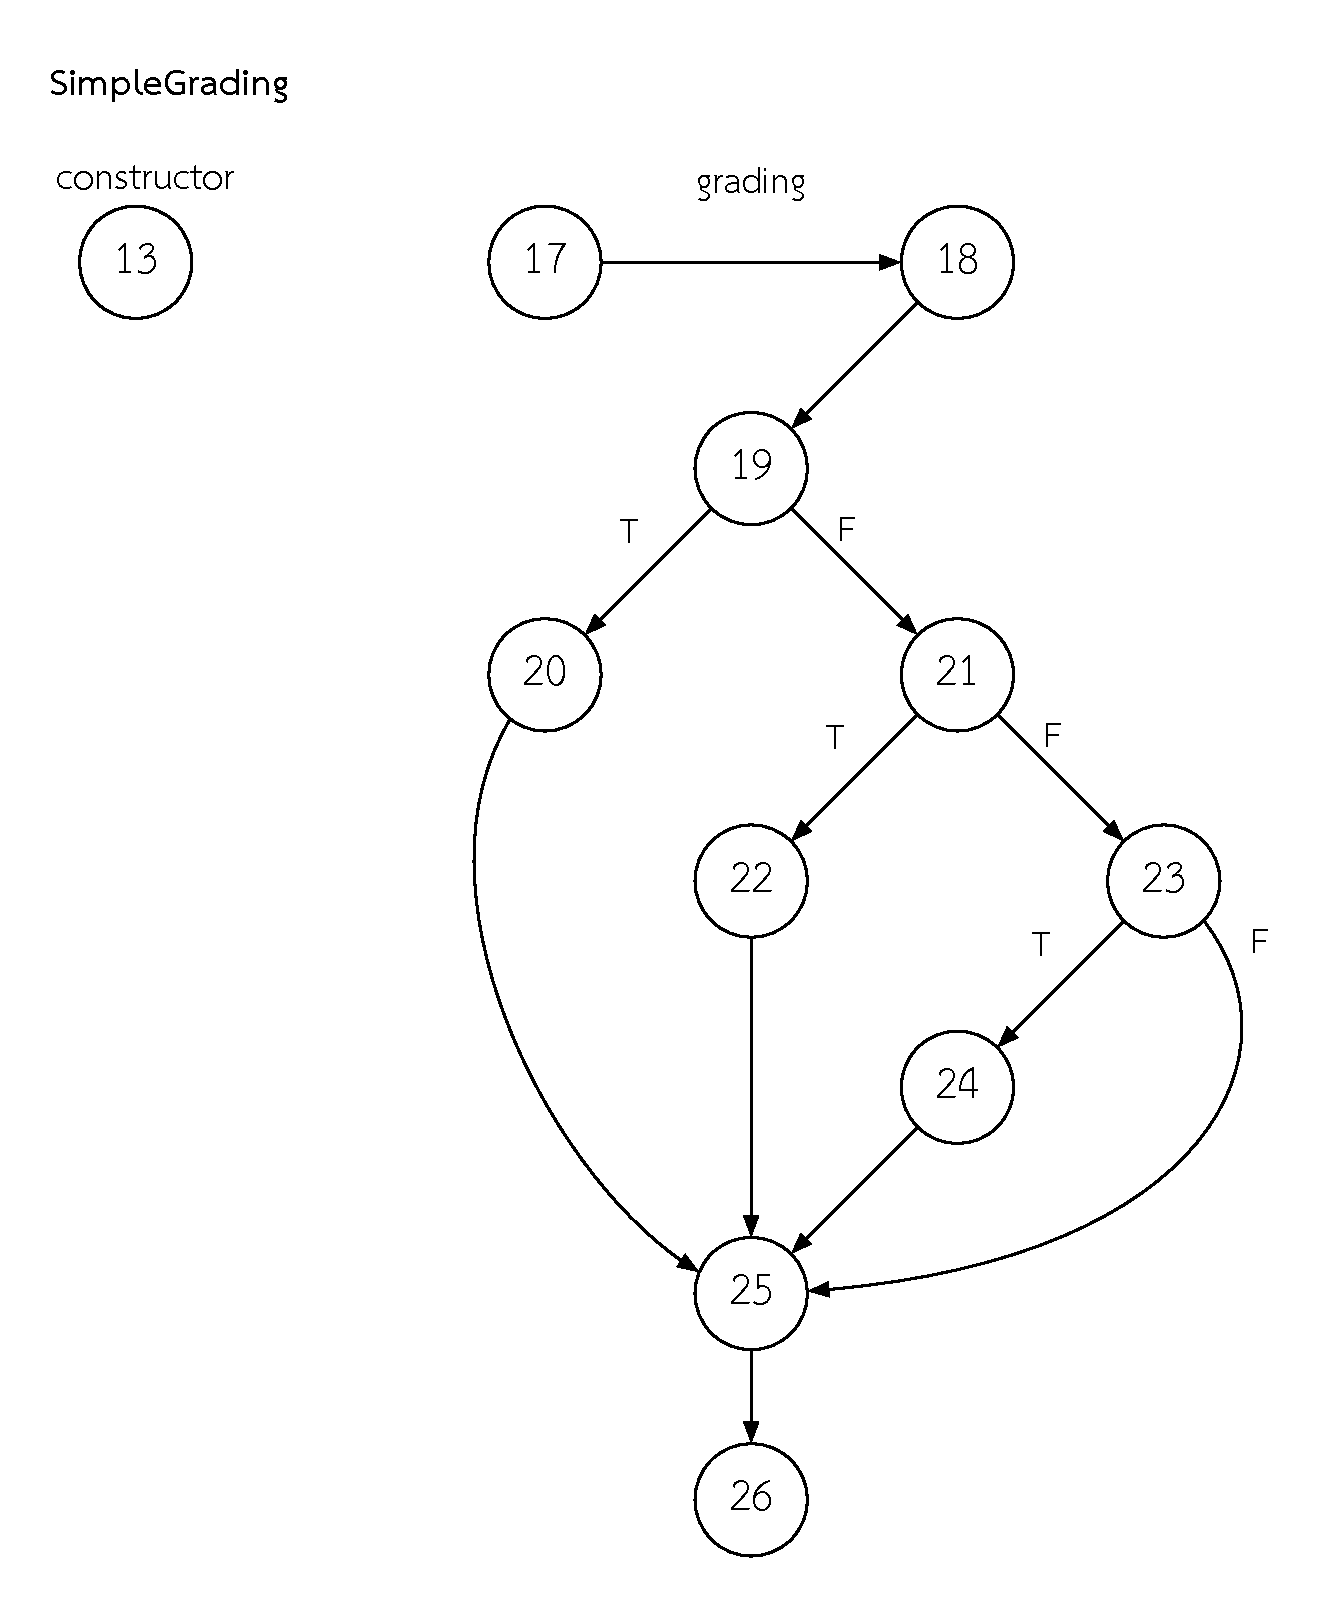
\includegraphics[width=0.7\textwidth]{cfg-SimpleGrading}
    \caption{{\cfg}สำหรับ{\class}คำนวณเกรดของนิสิต}
    \label{fig:cfgSimpleGrade}
\end{figure}

\subsubsection{การวิเคราะห์พารามิเตอร์และการคืนค่าของ{\method} (5.2)}

แนวทางในขั้นตอนนี้จะนำ{\TestPath}ที่ได้คัดเลือกไว้ในขั้นตอนก่อนหน้านี้ (ซึ่งในที่นี้คือ\tabpageref{tab:testPath}) มาพิจารณาข้อมูลนำเข้า
และพารามิเตอร์ของแต่ละ{\method}ที่มีการเรียกผ่านกัน โดยจะเริ่มพิจารณาที่{\PredicateNode}ที่อยู่ในลำดับท้ายสุดของ{\TestPath}ก่อนเสมอ 
แล้วจึงนำเงื่อนไขการสร้างข้อมูลของทั้งเส้นทางมากำหนดกรอบสำหรับการสร้างข้อมูล 
ยกตัวอย่างเช่น {\TestPath}สำหรับ{\class} \code{SimpleGrading} (\tabpageref{tab:testPath}) พบว่ามี{\PredicateNode} ณ {\Node} 19
{\TestPath} มีเงื่อนไข student\_score < SCORE\_MINIMUM\_STATISFIED หรือ student\_score < 80 

นอกจากนั้นแล้วยังพบ{\PredicateNode}ใน{\TestPath}ของ \code{SimpleBonusScore} นั้น
พบว่ามี{\PredicateNode} ณ {\Node} 8, 9 และ 11 ซึ่งมีเงื่อนไข ดังนี้

\begin{enumerate}
    \item[8:] \code{bonus\_score > 0} \label{itm:bonusscore}
    \item[9:] \code{student\_score <= 50} \label{itm:studentscore}
    \item[11:] \code{this.quiz.getQuizScore(student\_id) < 20} \label{itm:studentid}
\end{enumerate}

เมื่อนำเงื่อนไขทั้งหมดมาพิจารณาร่วมกันจะได้กรอบค่าของ{\it พารารมิเตอร์ที่น่าจะเป็นไปได้ (ช)} ดังตาราง
\begin{table}[ht!]
    \centering
    \caption{ค่าของพารามิเตอร์ที่น่าจะเป็นไปได้ (ช) ตามเงื่อนไขที่พบทั้งหมดบน{\TestPath}}
    \label{tab:caseIllustrate}
    \begin{tabular}{|l|c|c|}
        \hline
                                & \code{student\_score} & \code{bonus\_score} \\ \hline
        \code{SimpleGrading}    & < 80                  & - \\ \hline
        \code{SimpleBonusScore} & >= 50                 & > 0 \\ \hline
    \end{tabular}
\end{table}

% 
% 
% ซึ่งจากเงื่อนไขด้านบนสามารถสร้างข้อมูลนำเข้าได้ คือ {\bf "bonus\_score = 0"} และ {\bf "student\_score = 50"} โดยเงื่อนไขใน{\Node}ที่ 11 
% นั้น{\method} \code{getQuizScore} จำเป็นต้องสุ่มข้อมูลเพื่อป้อนให้กับ \code{student\_id} โดยนำเข้อมูล
% 
% บน{\TestPath}นี้มีเงื่อนไข student\_score < SCORE\_MINIMUM\_STATISFIED หรือ student\_score < 80 

\subsubsection{สุ่มข้อมูลนำเข้าสำหรับเมธอด (5.3)}

สำหรับแนวทางการดำเนินงานในขั้นตอนนี้จะรับกรอบการการสร้างข้อมูลนำเข้าจากกระบวนการก่อนหน้าเพื่อนำมาสร้างข้อมูลทดสอบ 
หากมีพารามิเตอร์ที่ไม่ปรากฎใน{\TestPath}เป็นข้อมูลนำเข้า ให้คำนวณหาค่าความน่าจะเป็นที่จะนำค่าคงที่ที่ได้จากขั้นตอนการ 
{\bf ทำเหมืองข้อมูลค่าคงที่ (2)} มาร่วมสร้างเป็นข้อมูลนำเข้าแทน จากตัวอย่างข้างต้น สามารถกำหนดกรอบ การสร้างข้อมูลนำเข้าสำหรับตัวแปร 
\code{student\_score} และเมื่อพิจารณาจากประเภทข้อมูลของ \code{student\_score} ได้ว่า ค่าที่สุ่มขึ้นมาได้นั้นต้องเป็นจำนวนเต็ม (Integer) 
ซึ่งอยู่ระหว่าง 50 - 79 และ \code{bonus\_score} จะต้องเป็นจำนวนเต็มที่มีค่ามากกว่า 0 เสมอ

สำหรับข้อมูลนำเข้าที่ไม่ปรากฎใน{\PredicateNode}บน{\TestPath}นั้นจะใช้การสุ่มค่าโดยใช้ค่าคงที่ที่ได้จากขั้นตอน {\bf ทำเหมืองข้อมูลค่าคงที่ (A)} 
เป็นข้อมูลเบื้องต้นในการสุ่มค่า 

กำหนดให้ค่าที่สุ่ม{\it ข้อมูนำเข้าสำหรับ{\method} (ช)} ได้ออกมาเป็นดัง \tabpageref{tab:GRTRandom}

\begin{table}[ht!]
    \centering
    \caption{ข้อมูลนำเข้าที่สุ่มได้}
    \label{tab:GRTRandom}
    \begin{tabular}{|l|c|c|}
        \hline
        ตัวแปร                    & ประเภทข้อมูล   & ค่าที่สุ่มได้          \\ \hline
        \code{student\_score}    & {\it int}    & {\bf 65}         \\ \hline
        \code{bonus\_score}      & {\it int}    & {\bf 42}         \\ \hline
        \code{student\_id}       & {\it String} & {\bf "IUUUSISS"} \\ \hline
    \end{tabular}
\end{table}

\newpage
\subsubsection{สร้างกรณีทดสอบ (5.4)}

ในขั้นตอนนี้จะนำข้อมูลนำเข้าที่สร้างจากกระบวนการก่อนหน้ามาสร้างกรณีทดสอบสำหรับภาษาจาวา โดยใส่ค่าคาดหวัง (บรรทัดที่ 7) 
จะเกิดจากการสุ่มโดยอิงตามประเภทข้อมูลที่{\method}นั้นคืนค่า ดังตัวอย่างของกรณีทดสอบภายใน {\it ชุดทดสอบ (ฌ)} ด้านล่าง

\begin{figure}[hbt!]
    \lstset{basicstyle=\small,style=thesiscodestyle}
    \lstinputlisting[language=Java]{methodology/SimpleGradingTest.java}
    \caption{กรณีทดสอบที่สร้างขึ้นจากข้อมูลทดสอบ}
    \label{fig:junitGradingTest}
\end{figure}

\subsection{การปรับค่าความคาดหวัง (6)}

แนวทางการดำเนินงานในขั้นตอนนี้จะเป็นการปรับค่าข้อมูลที่อยู่ภายในกรณีทดสอบที่ได้รับโดยนักทดสอบซอฟต์แวร์ เพื่อให้กรณีทดสอบนั้นสอดคล้องกับการทำงานที่ควรจะเป็นของโปรแกรม
มากที่สุด เนื่องจากการวิจัยครั้งนี้ยังไม่รองรับการวิเคราะห์ค่าผลลัพธ์ที่ได้จากการดำเนินงานของ{\method} ยกตัวอย่างเช่นกรณีทดสอบที่ได้จากขั้นตอนที่ 5.4 
ดัง \figref{fig:junitGradingTest} เมื่อได้ปรับการปรับค่าความคาดหวังจากนักทดสอบซอฟต์แวร์แล้วจะได้เป็นดัง{\figref{fig:junitGradingTestRefined}
ซึ่งในที่นี้นักทดสอบซอฟต์แวร์ได้ปรับค่าในบรรทัดที่ 5 โดยเปลี่ยนจาก \code{"IUUUSISS"} ให้เป็นค่า \code{"5873000021"} 
และบรรทัดที่ 6 คือค่า \code{"lorem"} เป็นค่า \code{"U"} จะได้ตัวอย่างของ {\it กรณีทดสอบพร้อมใช้งาน (ญ)} ดังนี้

\begin{figure}[hbt!]
    \lstset{style=thesiscodestyle}
    \lstinputlisting{methodology/SimpleGradingTest-Refined.java}
    \caption{กรณีทดสอบที่สร้างขึ้นจากข้อมูลทดสอบที่ปรับค่าจากนักทดสอบซอฟต์แวร์แล้ว}
    \label{fig:junitGradingTestRefined}
\end{figure}

\subsection{การทดสอบซอฟต์แวร์ (7)}

แนวทางการดำเนินงานในขั้นตอนนี้จะรับ {\it ชุดกรณีทดสอบ (ญ)} เข้าทดสอบร่วมกับ{\sourcecode}ที่ผ่าน{\it การแทรกคำสั่ง (จ)} จาก{\it ฐานข้อมูล (A)} 
และรวบรวมข้อมูลที่เกิดจากชุดคำสั่งที่แทรกไว้ ซึ่งปรากฎขึ้นระหว่างการทดสอบเข้าไว้ด้วยกันเป็น {\it ผลลัพธ์การทดสอบซอฟต์แวร์ (ฎ)} 
เพื่อใช้ตรวจสอบให้แน่ใจว่ากรณีทดสอบนั้นสามารถทดสอบ{\TestPath}ที่เลือกได้ 

\subsection{เปรียบเทียบผลลัพธ์การดำเนินงาน (8)}

ในขั้นตอนนี้จะรับ {\it ผลลัพธ์การทดสอบซอฟต์แวร์ (ฎ)} มาสร้างเส้นทางการทดสอบเทียบกับ{\TestPath}ที่ได้เลือกไว้ก่อนหน้านี้ 
เพื่อให้แน่ใจได้ว่าชุดทดสอบที่สร้างขึ้นนั้นครอบคลุม{\scg}ตาม{\TestPath}ที่กำหนดไว้
